% !TeX encoding = UTF-8
% !TeX spellcheck = pt_BR
% !TeX root = 2024-JOAO-FERREIRA-TESE.tex
%---------------------------------------------------------------------

%---------------------------------------------------------------------
% Tese de Doutorado
% Autor: João Ferreira da Silva Júnior
%---------------------------------------------------------------------



%---------------------------------------------------------------------
%---------------------------------------------------------------------
%---------------------------------------------------------------------
%---------------------------------------------------------------------
%---------------------------------------------------------------------
%---------------------------------------------------------------------
%---------------------------------------------------------------------
%---------------------------------------------------------------------
%---------------------------------------------------------------------
%---------------------------------------------------------------------
\chapter[Introdução]{Introdução}\label{cha:introducao}
    \chapterprecishere{
        \hspace{.2\textwidth}
        \hspace*{\fill}
        \begin{minipage}{.6\textwidth}
            \SingleSpace
            \raggedleft
            \noindent
            ``A luz sempre encontrará aqueles que a procuram.''\\
            (Autor desconhecido)
            % \emph{}
        \end{minipage}
    }
    \lipsum[1]
%---------------------------------------------------------------------



%---------------------------------------------------------------------
%---------------------------------------------------------------------
%---------------------------------------------------------------------
%---------------------------------------------------------------------
%---------------------------------------------------------------------
% \vspace*{0.2cm}
\section[Subseção 1]{Subseção 1}\label{sec:introducao-subsecao1}
    \lipsum[1]
%---------------------------------------------------------------------



%---------------------------------------------------------------------
% \vspace*{0.2cm}
\subsection[Sub-subseção 1]{Sub-subseção 1}\label{subsec:introducao-subsubsecao1}
    \lipsum[1]

    A seguir dois exemplos de tabela baseados no modelo do IBGE, o primeiro utilizado uma imagem para apresentar os dados, na \autoref{tab:pokemon-imagem}, e o segundo exemplo de fato trazendo os dados no formato de tabela, na \autoref{tab:pokemon-tabela}.
    \begin{table}[htb]
        \IBGEtab{%
            \caption{Trilha Sonora Pokémon --- em imagem}\label{tab:pokemon-imagem}
        }
        {%
            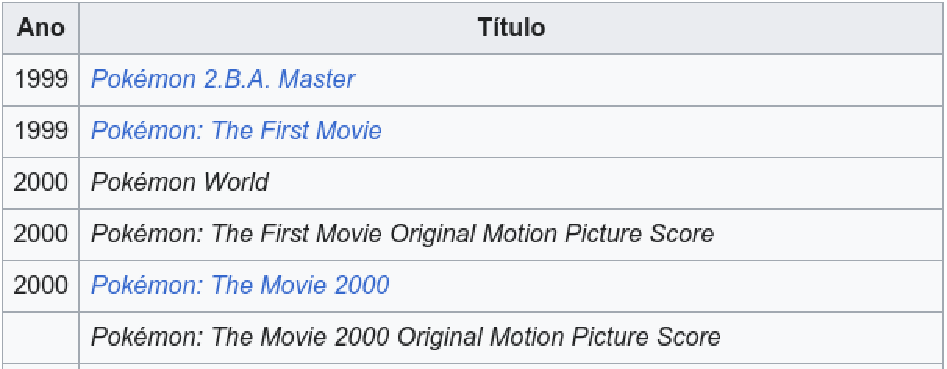
\includegraphics[width=0.8\textwidth,keepaspectratio]{img/01-introducao/pokemon.pdf}
        }
        {%
            \fonte{Adaptado de \citeonline{Wikipedia2005}.}
        }
    \end{table}

    \begin{table}[htb]
        \IBGEtab{%
            \caption{Trilha Sonora Pokémon --- em tabela}\label{tab:pokemon-tabela}
        }
        {%
            \begin{tabular}{cl}
                \toprule
                \textbf{Ano}    & \textbf{Título}                                           \\
                \midrule\midrule
                1999            & Pokémon 2.B.A. Master                                     \\
                1999            & Pokémon: The First Movie                                  \\
                2000            & Pokémon World                                             \\
                2000            & Pokémon: The First Movie Original Motion Picture Score    \\
                2000            & Pokémon: The Movie 2000                                   \\
                                & Pokémon: The Movie 2000 Original Motion Picture Score     \\
                \bottomrule
            \end{tabular}
        }
        {%
            \fonte{Adaptado de \citeonline{Wikipedia2005}.}
        }
    \end{table}

    Também é possível utilizar parágrafos dentro da tabela para posicionar os dados, que ficarão automaticamente alinhados à esquerda.
    \begin{table}[htb]
        \IBGEtab{%
            \caption{Trilha Sonora Pokémon --- em tabela com parágrafo}\label{tab:pokemon-tabela-paragrafo}
        }
        {%
            \begin{tabular}{cp{13.0cm}}
                \toprule
                \textbf{Ano}    & \textbf{Título}                                           \\
                \midrule\midrule
                1999            & Pokémon 2.B.A. Master                                     \\
                1999            & Pokémon: The First Movie                                  \\
                2000            & Pokémon World                                             \\
                2000            & Pokémon: The First Movie Original Motion Picture Score    \\
                2000            & Pokémon: The Movie 2000                                   \\
                & Pokémon: The Movie 2000 Original Motion Picture Score     \\
                \bottomrule
            \end{tabular}
        }
        {%
            \fonte{Adaptado de \citeonline{Wikipedia2005}.}
        }
    \end{table}

%---------------------------------------------------------------------



%---------------------------------------------------------------------
%---------------------------------------------------------------------
%---------------------------------------------------------------------
%---------------------------------------------------------------------
%---------------------------------------------------------------------
% \vspace*{0.2cm}
\section[Subseção 2]{Subseção 2}\label{sec:introducao-subsecao2}
    \lipsum[1]

    \begin{figure}[htb]
        \centering
        \caption{Hybrid Artificial Neural Network}\label{fig:hybrid-artificial-nn}
        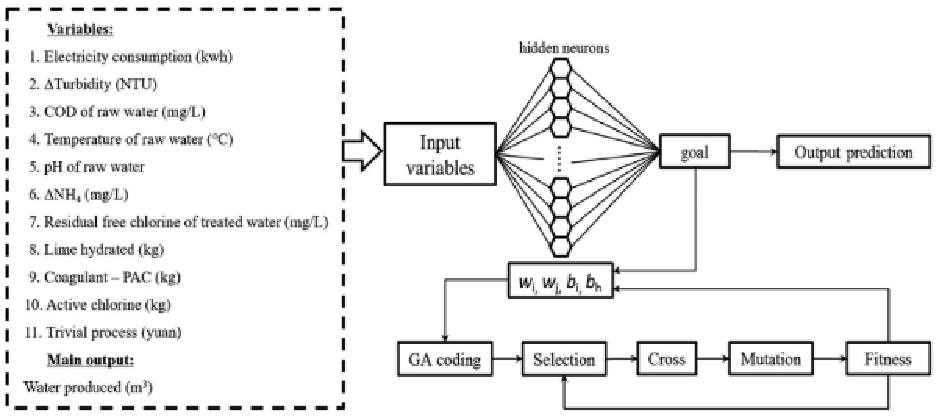
\includegraphics[width=0.8\textwidth,keepaspectratio]{img/01-introducao/hybrid-artificial-nn.pdf}
        %
        \fonte{Adaptado de \citeonline{Zhang2019}.}
        %
        % \nota[]
        \nota[]{%
            \parbox{0.8\textwidth}{%
                Aqui segue uma nota explicativa sobre o conteúdo e propósito da imagem.
            }
        }
    \end{figure}

    \lipsum[2]

    \lstinputlisting[%
        label=codigo-python,
        caption=codigo-python,
        language=Python,
        basicstyle=\tiny\ttfamily, breakatwhitespace=false,
        breaklines=true, breakatwhitespace=false, prebreak=\space, postbreak=\space
        showspaces=false, showstringspaces=false, showtabs=false,
        frame=single, rulecolor=\color{gray}, keywordstyle=,
        numbers=left, numbersep=5pt, numberstyle=\tiny\color{gray}, stepnumber=1
    ]{inc/codigo-python.py}

%---------------------------------------------------------------------